%!TEX encoding = UTF-8 Unicode

\section{関連研究}

\subsection{緒言}
本章では関連研究について述べる.はじめに,一般的なHPCシステムの利用方法について説明する.続いて,関連研究であるOpen OnDemandと呼ばれるウェブインタフェースについて説明する.ウェブインタフェースの機能やその設計について説明し,既存のウェブインタフェースの利点を整理する.最後に,既存のウェブインタフェースにおける課題を述べる.

\subsection{HPCシステム利用方法}
HPCシステムとは,コンピュータクラスタの能力を利用して,デスクトップ型コンピュータやノートブック型コンピュータを遥かに凌ぐ速度で計算課題 (ジョブ)を処理し,実行するシステムを指す.このような計算能力の集約によって,様々な科学分野において他の方法では対処できない大きな課題を解決できる.実際に,平均的なデスクトップ型コンピュータは毎秒数十億の浮動小数点演算を実行できる.しかし,HPCシステムは,1秒に数千兆の計算を実行することができることが知られている.例えば,スーパーコンピュータ京は1秒間に約1京回,スーパーコンピュータ富岳は1秒間に約44京回の浮動小数点演算を行うことができる\cite{kei,hugaku}.そのため,大規模な計算に対して,HPCシステムの利用は効果的であるといえる.\par
一般的なHPCシステムの利用の流れを図\ref{fig4}に示す.HPCシステムは数種類のサーバやデータベースから構成される.HPCシステムには,ジョブを実行するために計算を行う計算サーバ (ワーカーノード),ワーカーノードを管理するためのジョブスケジューラが配備されたジョブ管理サーバ (マスターノード),ユーザ情報が保存されたデータベースと連携してログイン情報の管理やユーザリクエストの受け渡しを行うログイン用サーバ,実行するジョブの入出力ファイルなどが保存されたファイル管理用サーバなどが存在する.\par
また,ジョブの実行を依頼するためにはジョブスクリプトファイルを作成する必要がある.ジョブスクリプトファイルとは,ジョブ投入用のシェルスクリプトファイルを指す.ジョブスクリプトファイルは大きく2つの部分で構成され,利用する計算機のリソースや環境を指定する部分と計算機に実行させる処理を記述する部分からなる.コード\ref{job_script}ではSLURMスケジューラのジョブスクリプトの例を示す.1行目はシェバンと呼称され,ファイルに記載されたプログラムが/bin/bashで実行されるということを明示的に記載している.2~6行目では,各ジョブスケジューラごとに定義されている接頭辞 (Slurmの場合は\#SBATCH)を用いて,利用する計算機のリソースや環境を指定する.2行目では,ジョブを投入するキューの名前を指定してる.3行目では,ジョブで使用するプロセス数を指定している.4行目では,実行するジョブの名前を指定している.5行目と6行目では,標準出力ファイルと標準エラー出力ファイルを指定している.なお,\%JはジョブIDに変換される.また,7行目は計算機に実行させる処理を記述する部分であり,プログラム (a.out)を実行する.\par
ユーザは利用したいHPCシステムを遠隔で操作するために自身のコンピュータからユーザ情報を用いて秘密鍵の登録を行った後,ログイン用サーバにSSH接続を用いてログインする.そして,ユーザは利用するジョブスケジューラの種類に応じた形式でジョブスクリプトを作成する.その後,各ジョブスケジューラごとに異なるユーザはジョブの実行を依頼するためのコマンドを用いて,マスターノード上で動作しているジョブスケジューラにジョブの実行を依頼する.ジョブスケジューラはファイル管理用サーバから入力ファイルを受け取り,ワーカーノードはマスターノードの命令に従ってジョブの実行を行う.ジョブ実行時の標準出力,エラー標準出力はファイルに出力され,ジョブ実行後に実行結果を確認することができる.\par

\begin{figure}[tb]
    \centering
    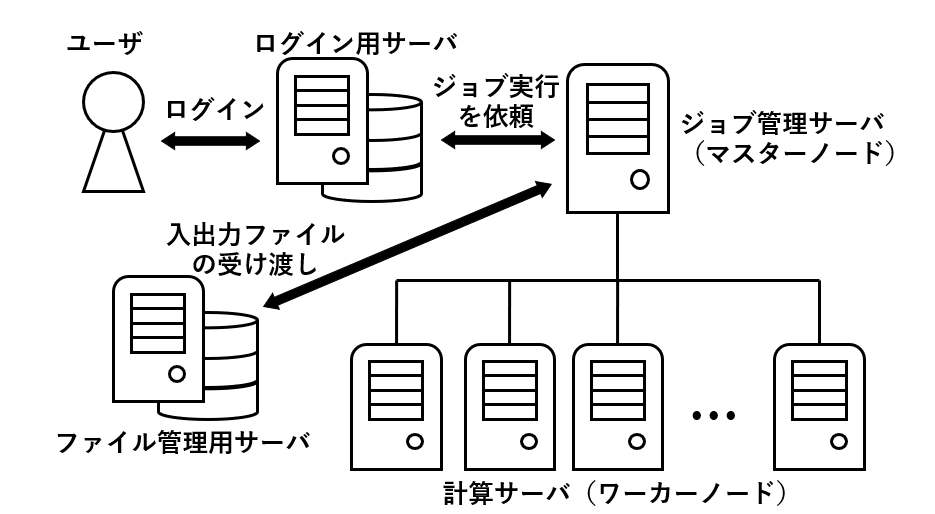
\includegraphics[width=120mm]{./fig/HPCsystem.png}
    \caption{一般的なHPCシステムの模式図}
    \label{fig4}
\end{figure}

\begin{lstlisting}[caption=Slurmのジョブスクリプトファイル作成例, label=job_script]

#!/bin/bash
#SBATCH -p partition1
#SBATCH -n 1
#SBATCH -J example
#SBATCH -o stdout.%J
#SBATCH -o stderr.%J
    
./a.out
    
\end{lstlisting}

\subsection{Open OnDemand}
代表的な関連研究として,Open OnDemand (OOD)とその機能や設計構成を紹介する\cite{cite2,cite3}.OODは米国オハイオ・スーパーコンピューティングセンターが開発したオープンソースソフトウェアであり,ウェブインタフェースを介してHPCシステムを利用できる環境を提供する.ユーザはウェブブラウザ上でHPCシステムを簡単に操作することができ,プラグインやほかのソフトウェアのインストールや設定は不要である.また,リモートデスクトップやJupyter Notebook\cite{jupyternotebook},Visual Studio Codeなどの対話的アプリケーションもウェブブラウザ上から利用することができる.OODは世界的に使われている様々なジョブスケジューラ (PBS Pro\cite{PBS_Pro},Slurm\cite{Slurm},Grid Engine\cite{Grid_Engine},Torque\cite{TORQUE},LSF\cite{LSF}など)に対応しているため,システム間の利用方法の差異を隠蔽している.\par
初めに,OODの機能について説明する.OODは,図\ref{dashboard}に示すダッシュボードと図\ref{homedirectory}に示すユーザのホームディレクトリを管理する画面,図\ref{activejobs}に示すジョブの状態を確認する画面,図\ref{jobcomposer}に示すジョブの管理を行う画面,図\ref{shell}に示すHPCクラスタのシェル操作を行う画面,開発者が任意の追加アプリケーションソフトウェアを導入することができるInteractive Apps画面から構成される.図\ref{homedirectory}に示すホームディレクトリ画面からはユーザのディレクトリを視覚的に操作することができ,ファイルやディレクトリの削除,追加,および編集なども容易に行うことができる.図\ref{activejobs}にはジョブの状態確認を行うActive Jobs画面を示す.ユーザは投入したジョブの状態をリアルタイムで確認することができる.図\ref{jobcomposer}のJob Composerの画面では,ユーザはジョブの作成,投入,削除などをすべてこの画面から行うことができ,HPCシステム内のジョブの管理を行うことができる.図\ref{shell}には,シェル画面を示す.ユーザは連携したHPCクラスタのシェルをウェブブラウザ上から操作することができる.このように,OODは様々な機能やアプリケーションソフトウェアと連携してHPCユーザの利用者支援を行っている.\par
続いて,OODの設計について説明する.OODのクラス図を図\ref{class_diagram}に示す.OODは現在多様なジョブスケジューラに対応しているが,各ジョブスケジューラへの対応はadaptersディレクトリ下に配置される.指定したジョブスケジューラに対応するために,各ジョブスケジューラ用のAdapterスーパークラスのサブクラスが宣言される.サブクラス内部ではジョブの投入を行うsubmitメソッド,クラスターの情報を取得するcluster\_infoメソッド,ユーザ情報を取得するaccountsメソッド,ジョブの情報を取得するinfoメソッド,info\_allメソッド,info\_where\_ownerメソッド,ジョブの状態を取得するstatusメソッド,ジョブの一時停止を行うholdメソッド,ジョブの再開を行うreleaseメソッド,ジョブの削除を行うdeleteメソッドなどが再定義されている.また,各ジョブスケジューラのサブクラス内にはBatchクラスが定義されており,前述したサブクラス内部のメソッドはBatchクラス内部のメソッドを利用して実装されている.例えば,AdapterスーパークラスのサブクラスであるSlurmクラスは,Slurmクラスタにジョブを投入するためのメソッドであるsubmitメソッドを再定義しており,Slurmクラスで定義されたsubmitクラスは内部クラスであるBatchクラスのsubmit\_stringメソッドを用いてジョブの投入を行う.このように,利用するジョブスケジューラのサブクラスで再定義されたメソッドを用いることで,OODは多様なジョブスケジューラに対応することができている.\par
以上のように,OODは視覚的かつ簡単な操作を用いてHPCシステムの利用を行うことができるというメリットを持つ.また,OODは対応しているジョブスケジューラごとにAdapterクラスが宣言されている.そのため,各Adapterクラスを新規作成および改修することで,OODのジョブスケジューラへの対応機能を改修することができる.そのため,多くのコンピューティングセンターで実用化され,OODのユーザ数も年々増加しており,HPC利用環境を提供するウェブインタフェースとして多くの研究開発が行われている.\par

\begin{figure}[t]
    \centering
    \fbox{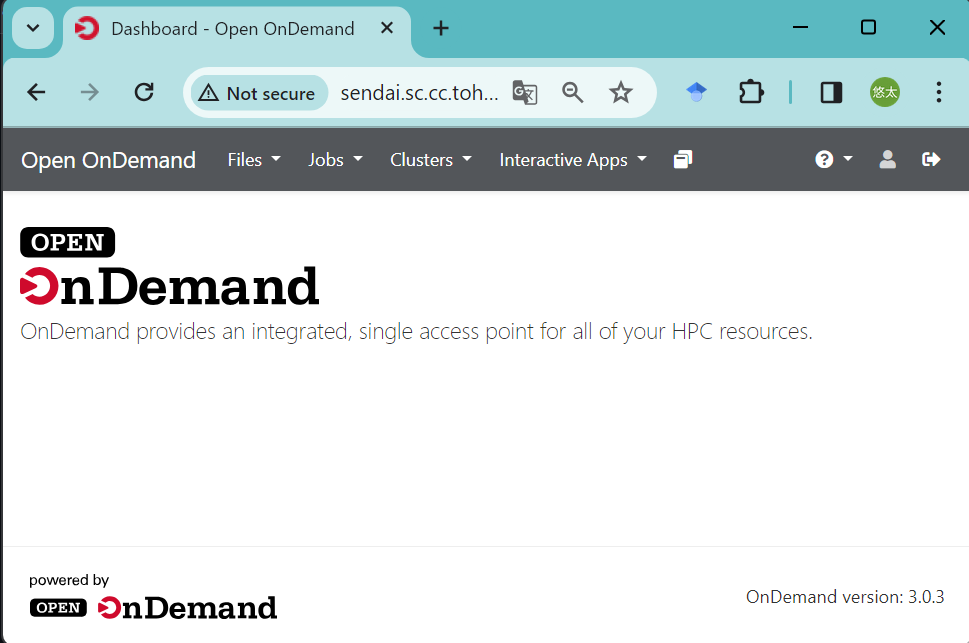
\includegraphics[width=120mm]{./fig/dashboard.png}}
    \caption{ダッシュボード画面}
    \label{dashboard}
\end{figure}

\begin{figure}[t]
    \centering
    \fbox{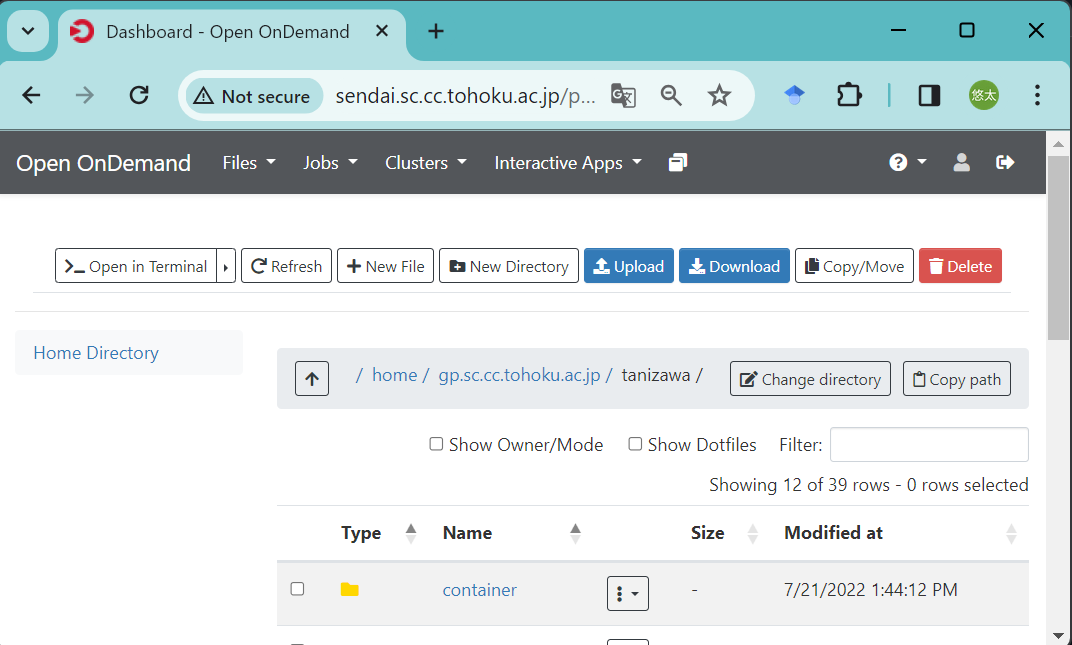
\includegraphics[width=120mm]{./fig/homedirectory.png}}
    \caption{ホームディレクトリ画面}
    \label{homedirectory}
\end{figure}

\begin{figure}[t]
    \centering
    \fbox{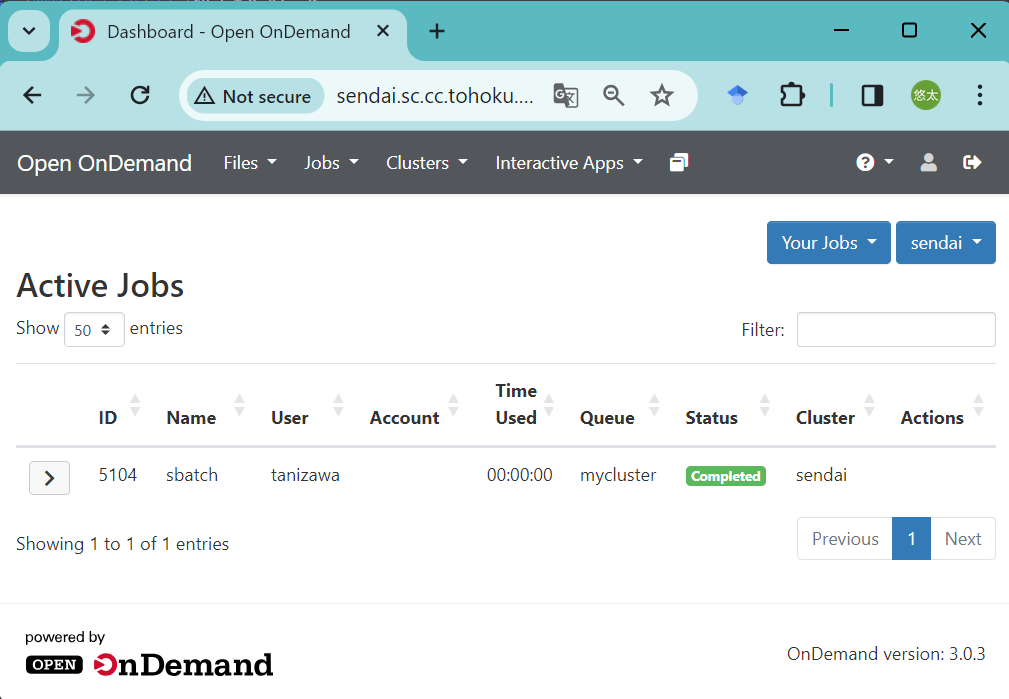
\includegraphics[width=120mm]{./fig/activejobs.png}}
    \caption{Active Jobs画面}
    \label{activejobs}
\end{figure}


\begin{figure}[b]
    \centering
    \fbox{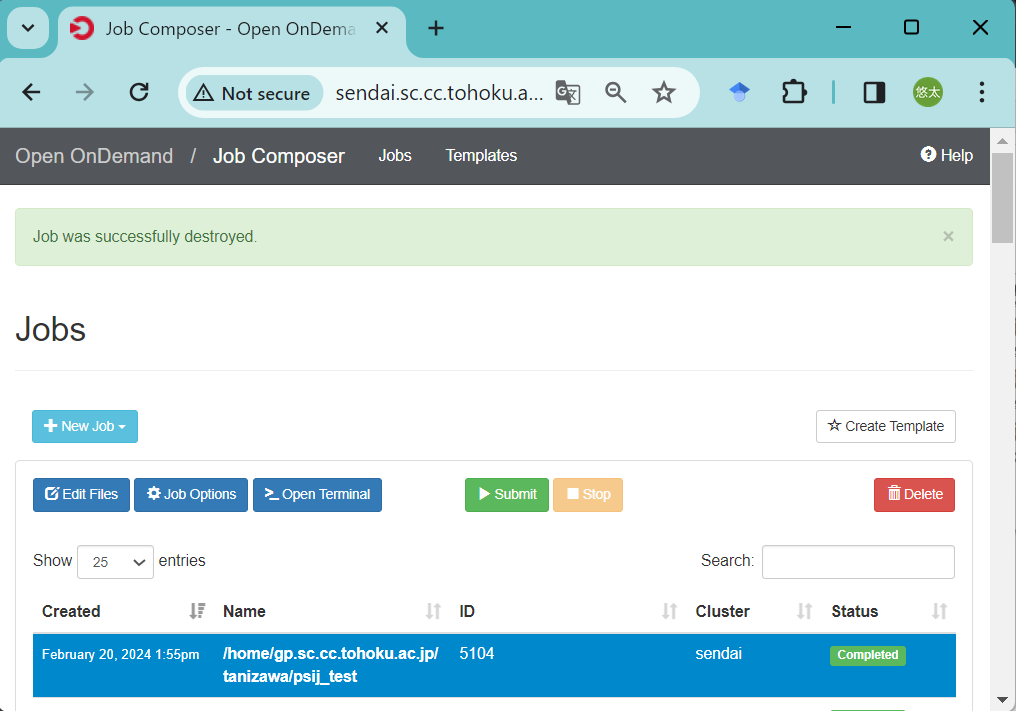
\includegraphics[width=120mm]{./fig/jobcomposer.png}}
    \caption{Job Composer画面}
    \label{jobcomposer}
\end{figure}

\begin{figure}[t]
    \centering
    \fbox{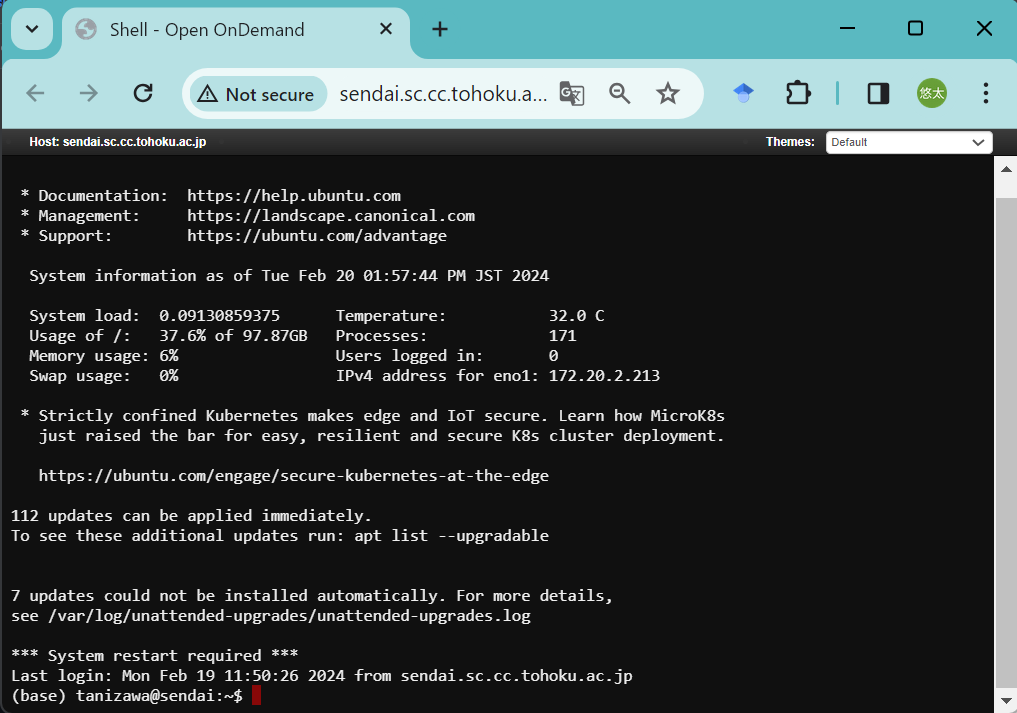
\includegraphics[width=120mm]{./fig/shell.png}}
    \caption{シェル画面}
    \label{shell}
\end{figure}

\begin{figure}[b]
    \centering
    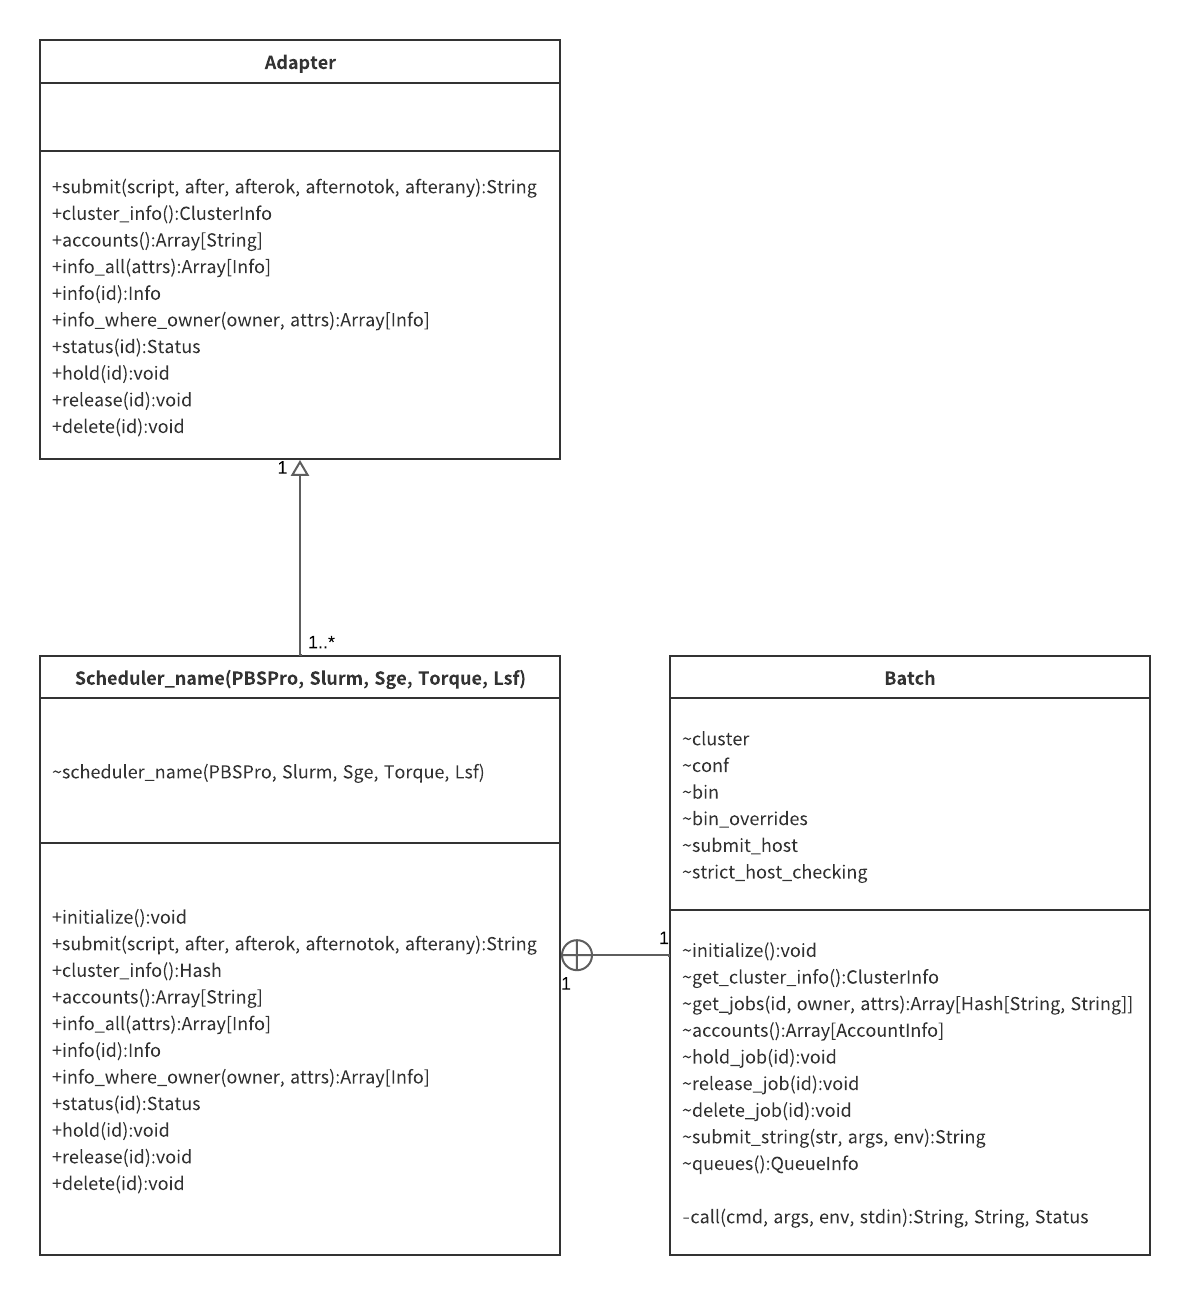
\includegraphics[width=120mm]{./fig/class_diagram.png}
    \caption{OODのクラス図}
    \label{class_diagram}
\end{figure}

\subsection{既存のウェブインタフェースにおける課題}
はじめに,既存のウェブインタフェースであるOODを介したHPCシステム利用環境について説明する.従来手法の模式図を図\ref{fig5}に示す.既存のウェブインタフェースは,各ジョブスケジューラと連携するための機能がウェブインタフェース本体と一体的に実装されている.また,OODはログイン時に認証機構を必要としており,DexとのOpeIDコネクト\cite{dex}\cite{openidconnect}やShibboleth\cite{shibboleth},CAS\cite{CAS}などの認証方法がある.OODは,前述した認証方法に必要な外部の認証用ディレクトリと連携してユーザ情報を管理することで,ウェブブラウザ上での利用空間の提供を行う.また,主要なジョブスケジューラの抽象化を行うことで,統一的な操作環境を提供する.\par

\begin{figure}[b]
    \centering
    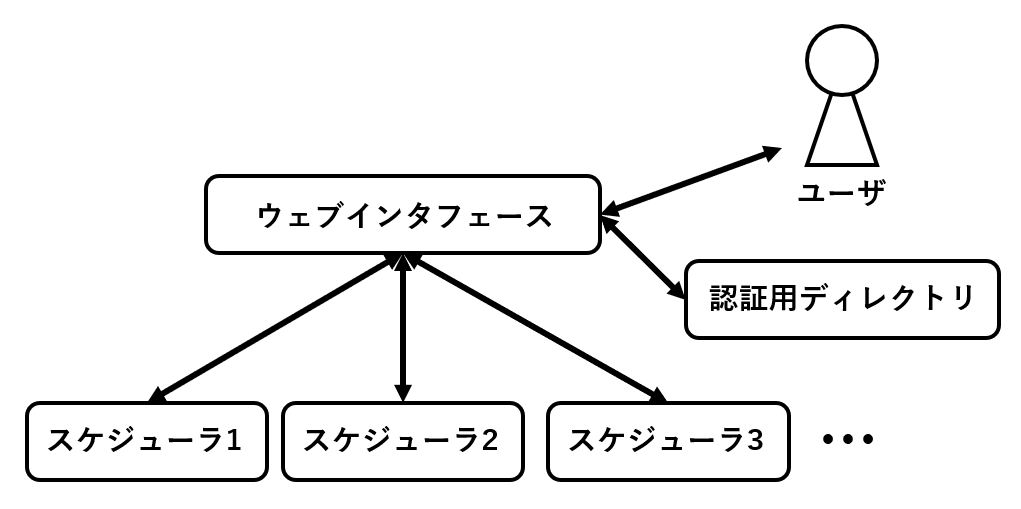
\includegraphics[width=120mm]{./fig/conventional_method.png}
    \caption{従来手法の模式図}
    \label{fig5}
\end{figure}

続いて,既存のウェブインタフェースにおける課題について説明する.OODは視覚的かつ簡単な操作を用いてHPCシステムの利用を行うことができるという利点を持っている.しかし,システム設計上の課題点も考えられる.\par
国内でのウェブインタフェースの実装事例として,スーパコンピュータ富岳でのOODの実装が挙げられる.OODは汎用的なツールであるが,富岳で用いられているジョブスケジューラ (Fujitsu Technical Computing Suite, Fujitsu TCS)に対応していなかったことから,中尾らはOODをFujitsu TCS向けに改修した事例を報告している\cite{cite4}.改修ではAdapterスーパークラスで定義されている下記のメソッドをFujitsu TCS用に実装している.\par

\textbf{submit} ジョブの投入\par
\textbf{delete} ジョブの削除\par
\textbf{status} ジョブの状態を取得\par
\textbf{hold} ジョブの一旦停止\par
\textbf{release} ジョブの再開\par
\textbf{info} ジョブの情報を取得\par
\textbf{info\_all} 全ジョブの情報を取得\par
\textbf{cluster\_info} HPCシステムの情報を取得\par
\textbf{supports\_job\_arrays} バルクジョブのサポートの可否\par
\textbf{directive\_prefix} ジョブスケジューラで用いられる接頭辞の取得 (Fujitsu TCSの場合はPJM)\par

さらに,本来OODに対応しているジョブスケジューラでは図\ref{activejobs}に示すActive Jobs画面のID番号の左にあるボタンをクリックすると,ジョブの詳細情報が表示される.しかし,Fujitsu TCSのようなOODに未対応であるジョブスケジューラは,ジョブの詳細が表示されない.そこで中尾らはFujitsu TCS用に詳細情報が表示されるようにActive Jobs画面の改修を行ったことも報告している\cite{cite4}.\par
ほかにも様々なジョブスケジューラが存在し,今後も登場することを考えると,ジョブスケジューラがの種類が増えるごとにOOD本体を直接改修する方法では保守性に問題があるといえる.\par


\subsection{結言}
本章では,関連研究について述べた.はじめに一般的なHPCシステムの利用方法について説明した.HPCシステムの利用方法について説明し,基礎的な知識を解説した.その後,Open OnDemandと呼ばれるウェブインタフェースについてその機能と設計について説明した.OODを用いることによる影響は大きく,HPCシステムのユーザに多くの利点をもたらすことができると考えられる.また,内部の設計を理解することで,OODのジョブスケジューラへの対応機能の改修方法を理解することができた.最後に,既存のウェブインタフェースについて,国内でのOODの実装例を参考にして課題点を述べた.ユーザに快適なHPC利用空間を提供するという利点に反して,システムの保守性が課題点として挙げられる.次章では,本章で述べた既存のウェブインタフェースにおける課題である保守性を考慮した手法を提案し,その実装を行う.\par